\documentclass[10pt,twocolumn,letterpaper]{article}

\usepackage{cvpr}
\usepackage{times}
\usepackage{epsfig}
\usepackage{graphicx}
\usepackage{amsmath}
\usepackage{amssymb}
\usepackage{array}
\usepackage{xfrac}
\usepackage{amssymb}
%\usepackage{todonotes}
\usepackage{centernot}
\usepackage{textcomp}
\usepackage{blindtext}
\usepackage{centernot}
\usepackage{wasysym}
\usepackage{siunitx}
\usepackage[letterpaper]{geometry}
\usepackage{color}
%\usepackage[table]{xcolor}
\usepackage{amsfonts}
\usepackage{mathtools}
\usepackage{multirow}
\usepackage[small,it]{caption}
%\usepackage{titling}
%\usepackage{filecontents}
%\usepackage{titlesec}
\usepackage[section]{placeins}
%\usepackage[hidelinks]{hyperref}
%\usepackage{fancyhdr}
\usepackage{cancel}
%\usepackage{abstract}
\usepackage{minted}
\usepackage{widetext}
\usepackage[utf8]{inputenc}

\sisetup{output-exponent-marker=\textsc{e}}

\DeclareMathOperator*{\argmax}{arg\,max}
\DeclareMathOperator*{\argmin}{arg\,min}

\newcommand{\squishlist}{
 \begin{list}{$\bullet$}
  { \setlength{\itemsep}{0pt}
     \setlength{\parsep}{3pt}
     \setlength{\topsep}{3pt}
     \setlength{\partopsep}{0pt}
     \setlength{\leftmargin}{1.5em}
     \setlength{\labelwidth}{1em}
     \setlength{\labelsep}{0.5em} } }


\newcommand{\squishlisttwo}{
 \begin{list}{$\bullet$}
  { \setlength{\itemsep}{0pt}
    \setlength{\parsep}{0pt}
    \setlength{\topsep}{0pt}
    \setlength{\partopsep}{0pt}
    \setlength{\leftmargin}{2em}
    \setlength{\labelwidth}{1.5em}
    \setlength{\labelsep}{0.5em} } }

\newcommand{\squishend}{
  \end{list}  }
\footskip = 50pt
\setlength{\skip\footins}{10pt}

\newcommand*{\vertbar}{\rule[-1ex]{0.5pt}{3.0ex}}
\newcommand*{\horzbar}{\rule[.5ex]{2.5ex}{0.5pt}}

% Include other packages here, before hyperref.

% If you comment hyperref and then uncomment it, you should delete
% egpaper.aux before re-running latex.  (Or just hit 'q' on the first latex
% run, let it finish, and you should be clear).
\usepackage[breaklinks=true,bookmarks=false]{hyperref}

\cvprfinalcopy % *** Uncomment this line for the final submission

\def\cvprPaperID{****} % *** Enter the CVPR Paper ID here
\def\httilde{\mbox{\tt\raisebox{-.5ex}{\symbol{126}}}}

% Pages are numbered in submission mode, and unnumbered in camera-ready
%\ifcvprfinal\pagestyle{empty}\fi
\setcounter{page}{1}
\begin{document}

%%%%%%%%% TITLE
\title{Histograms of Oriented Gradients}

\author{Edgar A. Margffoy-Tuay\\
Universidad de los Andes\\
201412566\\
{\tt\small ea.margffoy10@uniandes.edu.co}
% For a paper whose authors are all at the same institution,
% omit the following lines up until the closing ``}''.
% Additional authors and addresses can be added with ``\and'',
% just like the second author.
% To save space, use either the email address or home page, not both
%\and
%Second Author\\
%Institution2\\
%First line of institution2 address\\
%{\tt\small secondauthor@i2.org}
}

\maketitle
%\thispagestyle{empty}

%%%%%%%%% ABSTRACT
\begin{abstract}
Histograms of Oriented Gradients (HOG) are image features that describe and capture local orientation information on an image. Reminiscent of SIFT features, HOG binarizes the gradient responses on a local window cell, which allow to describe local objects based on their gradient filter responses, based on this features, it is possible to distnguish different objects and eventually, detect them. The objective of the present report consists on designing and testing a multiscale object detector based on HOG features, similar to the baseline approach proposed by Dalal and Triggs adapted to face detection. 
\end{abstract}

%Segmentation represents one of the core Computer Vision tasks in scientfic and academic research since the 1970s, this problem is defined as the grouping of pixels on a image according to several semantic categories of interest. Until recently, this problem was approached by using pixel-level mathematical formulations based on classical image processing and DSP, without any association with other Computer Vision problems nor any AI-related task, such as NLP. However, after the rise of

%%%%%%%%% BODY TEXT
\section{Introduction}
%\subsection*{Context}
HOG features were proposed by Dalal and Triggs on \cite{1467360} to characterize and generalize pedestrian outlines and contour gradient orientations suitable to detect them on a street scene, initially, HOG descriptors were only employed on object categories that presented a similar geometry, point of view and aspect ratio, which favored the generalization of a single HOG activation template that could be applied onto a test image via convolution. Due to the similar geometry, aspect ratio and orientation present on pedestrian pictures, HOG representation was suitable to solve this binary classification problem, as Dalal and Triggs demostrated.
\\
\\
However, if simple HOG features were to be applied to solve a complex multiclass object that presents several of the initial HOG limitations such as viewpoint translation, geometric obfuscation and intra-class instance differences, the expected classification accuracy rate should be low, due to the introduction of several false positive detections due to the similarity between the HOG representations of different objects that should be represented differently. 
\\
\\
To solve those limitations, several HOG improvements were proposed, such as Deformable Part Models (DPM) \cite{felzenszwalb2010object}, on which not only a single local object HOG representation is used but also the relation with nearby HOG features. This approach allows to represent an object as a graph of HOG features, giving more information about geometry, location and viewpoint of an image. Another approach consists on training a single SVM classifier per each HOG object instance, this approach, denomined Exemplar SVMs \cite{malisiewicz2011ensemble}, allows not only to classify each object instance accurately, but it also allows to obtain geometrical information suitable to more advanced tasks, such as 3D reconstruction and pose estimation, however, this method is too expensive due to the formulation and minimization of a single classification model per each example present on the dataset, which means that this approach is not scalable, however it is highly parallel, due to the independence of each exemplar classification model. 
\\
\\
To explore the limitations of a plain HOG detector on a complex detection task, such as face detection, a simple Dalal-Triggs inspired framework is proposed to solve this task over the Wider Face detection dataset \cite{yang2016wider}, a modern state-of-the-art face detection benchmark.

\section{Materials and Methods}
HOG feature calculation is similar to SIFT \cite{Lowe:1999:ORL:850924.851523} representation, the main difference between both descriptors is related to gradient histogram normalization across a segmentation of a window on a set of blocks, this procedure allows to decorrelate gradient histograms on different blocks members of a single HOG window, which allows to introduce more redundancy onto the model, increasing the accuracy of the final classification model.
\\
\\
To detect multiple object instances on each image, a normalized sliding window of size $136 \times 100$ approach was used, this decision was taken taking in account all the possible aspect ratios of the bounding boxes present on the dataset, some of them are elogated, and other have a similar proportion. This window was also applied over different scales, to ensure that smaller background or near faces were also subject to examination. Finally, the detection pipeline was implemented without any addition nor any improvement such as DPMs or Exemplar SVMs. To calculate HOG histograms across each of the dataset images, a cell of size 8 was defined.
\\
\\
The model training was done using 5 iterations of hard negative mining, by selecting intial random regions present on all images
All the implementation was based upon Andrea's Vedaldi vlfeat and matconvnet libraries \cite{vedaldi08vlfeat}, as shown on the Oxford's VGG tutorial on object detection\footnote{Available at: \url{http://www.robots.ox.ac.uk/~vgg/practicals/category-detection/}}.  

\subsection*{About the Datasets}
\squishlist
\item \textbf{Wider Face}: This dataset contains 32203 images, which in turn contains 393703 annotated faces (Bounding boxes) grouped on 60 event categories. All detection evaluations are based on the Intersection-over-Union (IoU) metric.
\squishend
%\begin{figure*}[t]
%	\centering
%	%	\begin{center}
%	%\fbox{\rule{0pt}{2in} \rule{0.9\linewidth}{0pt}}
%	\epsfig{file=./Assets/Model_red.pdf,width=0.8\linewidth,clip=}
%	%\includegraphics[width=0.8\linewidth]{egfigure.eps}
%	%	\end{center}
%	\caption{Visual description of the planned baseline to approach the image segmentation recovery problem given a video input. Images taken by the author}
%	\label{Fig:F1}
%	%\label{fig:long}
%	%\label{fig:onecol}
%\end{figure*}


\section{Results}
\begin{figure}[H]
		\centering
		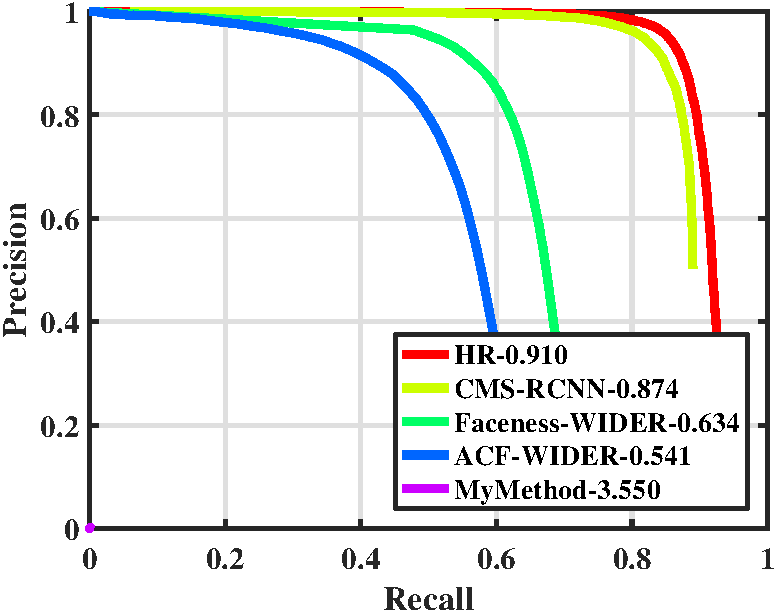
\epsfig{file=./results/PR.pdf,width=1.0\linewidth,clip=}
		\caption{Precision-Recall curve results of the HOG proposed model}
		\label{Fig:PR}
\end{figure}


As it can be shown on Figure~\ref{Fig:PR}, the proposed HOG detection model only outputs random bounding boxes, and it is no more different from a random 

{\small
\bibliographystyle{ieee}
\bibliography{egbib}
}


\newpage
%\section{Some Results}
%\begin{figure}[H]
%	\centering
%	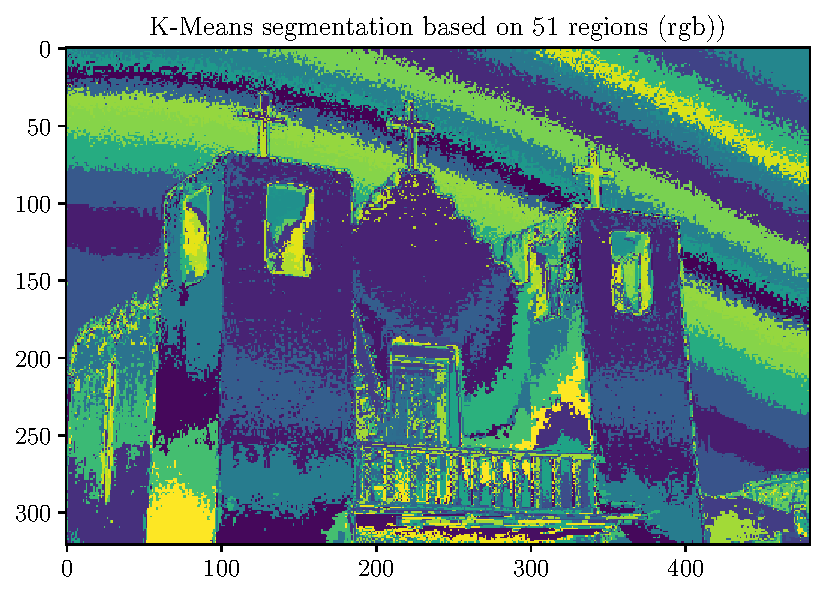
\epsfig{file=./Assets/24063_k-means_rgb_51.pdf,width=1.0\linewidth,clip=}
%	\caption{Example of K-Means segmentation result subject to 51 regions (No spatial)}
%	\label{Fig:kmeans1}
%\end{figure}
%
%
%\begin{figure}[H]
%	\centering
%	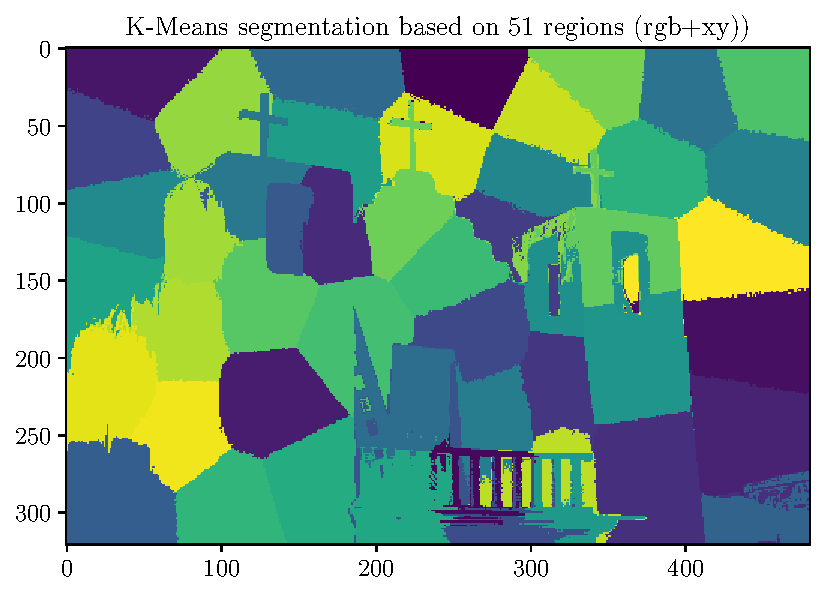
\epsfig{file=./Assets/24063_k-means_rgb+xy_51.pdf,width=1.0\linewidth,clip=}
%	\caption{Example of K-Means segmentation result subject to 51 regions (Spatial), this figure presents a large number of convex and spherical regions}
%	\label{Fig:kmeans2}
%\end{figure}
%
%\begin{figure}[H]
%	\centering
%	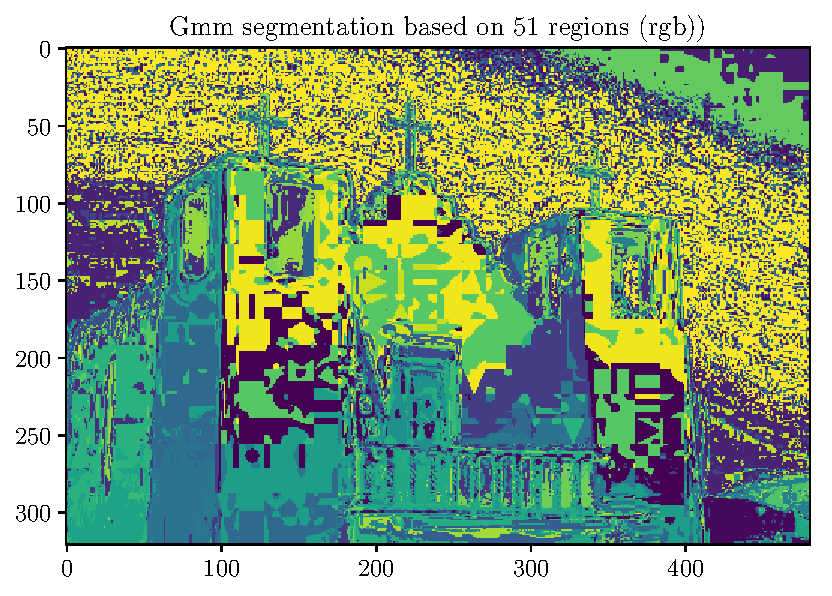
\epsfig{file=./Assets/24063_gmm_rgb_51.pdf,width=1.0\linewidth,clip=}
%	\caption{Example of GMM segmentation result subject to 51 regions (No spatial)}
%	\label{Fig:gmm1}
%\end{figure}
%
%\begin{figure}[H]
%	\centering
%	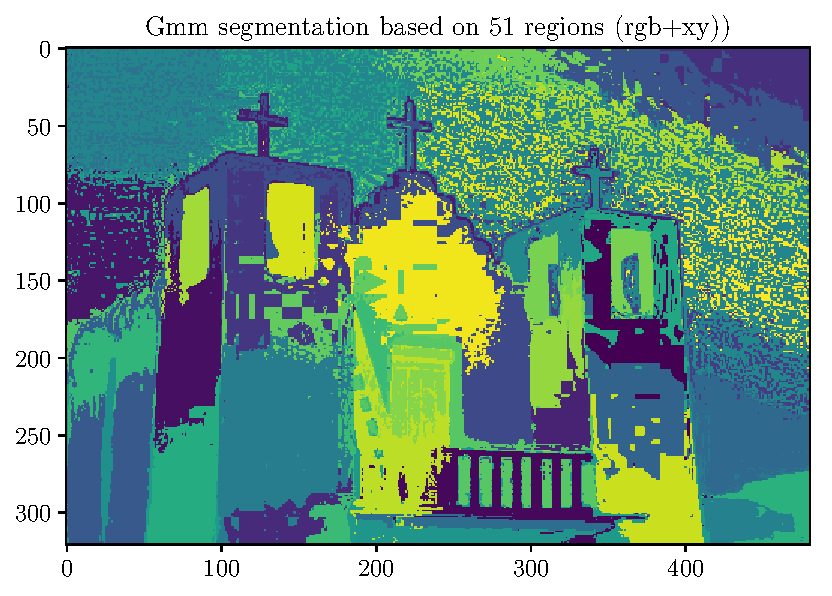
\epsfig{file=./Assets/24063_gmm_rgb+xy_51.pdf,width=1.0\linewidth,clip=}
%	\caption{Example of GMM segmentation result subject to 51 regions (Spatial information added), the noise was reduced}
%	\label{Fig:gmm2}
%\end{figure}
%
%\begin{figure}[H]
%	\centering
%	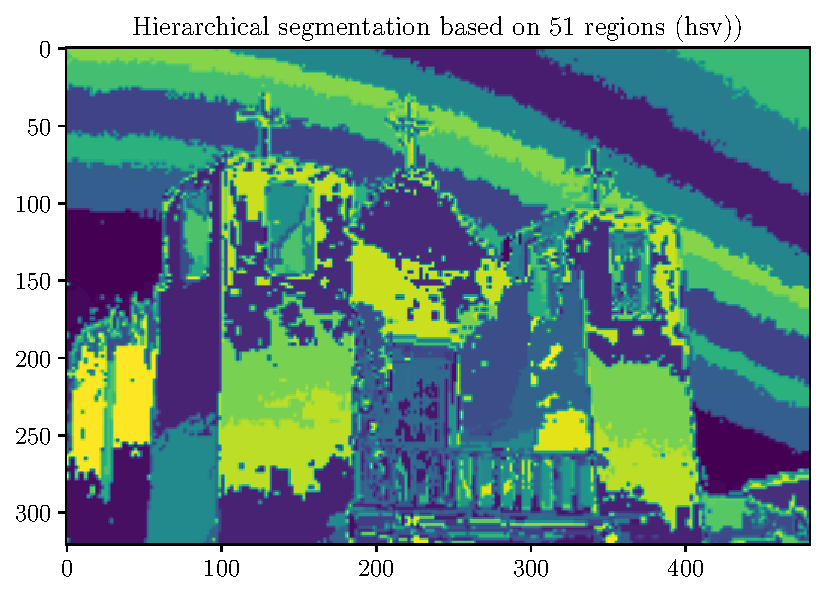
\epsfig{file=./Assets/24063_hierarchical_hsv_51.pdf,width=1.0\linewidth,clip=}
%	\caption{Example of Hierarchic segmentation result subject to 51 regions (No spatial information added), notice the smooth noise throughout all the regions by interpolation effects}
%	\label{Fig:hier1}
%\end{figure}
%
%\begin{figure}[H]
%	\centering
%	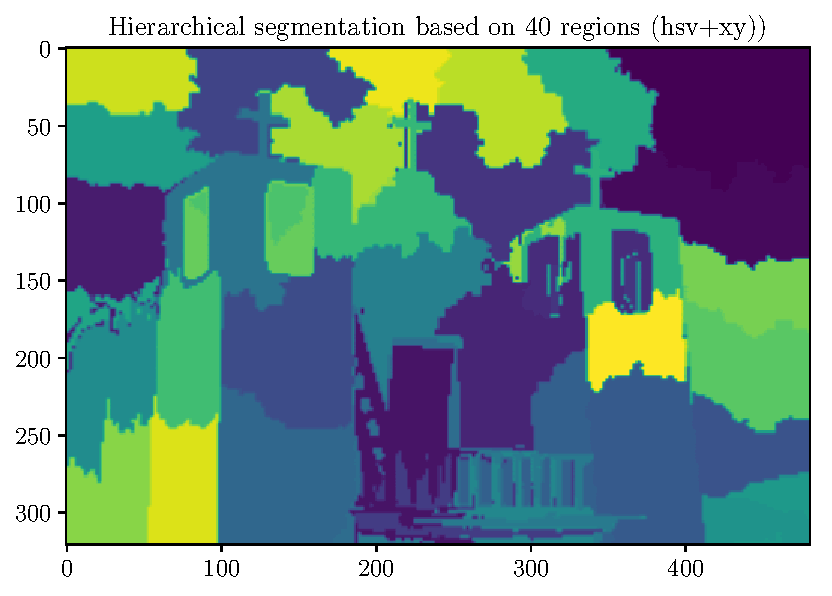
\epsfig{file=./Assets/24063_hierarchical_hsv+xy_40.pdf,width=1.0\linewidth,clip=}
%	\caption{Example of Hierarchic segmentation result subject to 40 regions (Spatial information added), notice the smooth noise throughout all the regions by interpolation effects}
%	\label{Fig:hier2}
%\end{figure}
%
%\begin{figure}[H]
%	\centering
%	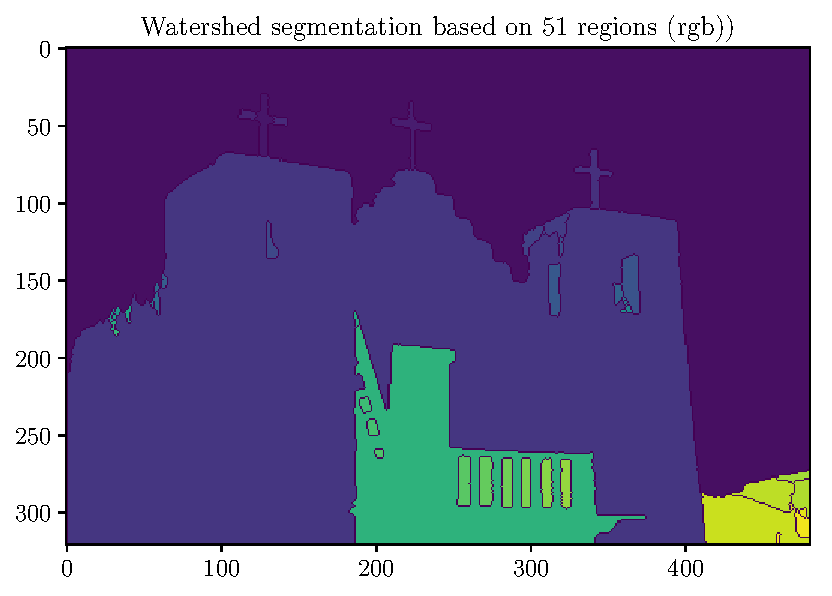
\epsfig{file=./Assets/24063_watershed_rgb_51.pdf,width=1.0\linewidth,clip=}
%	\caption{Example of H-Minima Watershed segmentation result subject to 51 regions, notice the well defined contours and regions}
%	\label{Fig:water1}
%\end{figure}
%
%\begin{figure}[H]
%	\centering
%	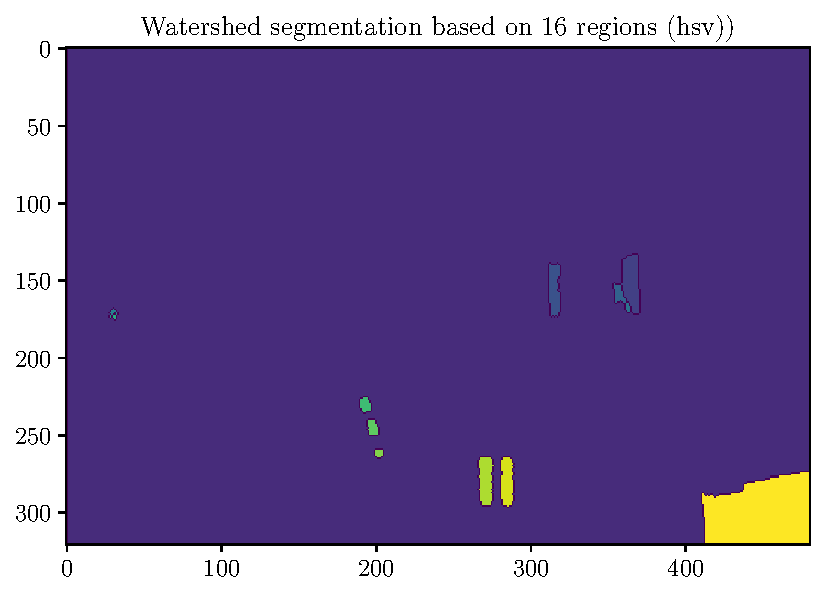
\epsfig{file=./Assets/24063_watershed_hsv_16.pdf,width=1.0\linewidth,clip=}
%	\caption{Example of H-Minima Watershed segmentation result subject to 16 regions, notice the disappearance of the main ROI}
%	\label{Fig:water2}
%\end{figure}



\end{document}
